%%%%%%%%%%%%%%%%%%%%%%%%%%%%%%%%%%%%%%%%%%%%%%%%%%%%%%%%%%%%%%%%%%%%%%%%%%%%%%%
% intro.tex: Introduction to the thesis
%%%%%%%%%%%%%%%%%%%%%%%%%%%%%%%%%%%%%%%%%%%%%%%%%%%%%%%%%%%%%%%%%%%%%%%%%%%%%%%%
\chapter{Introduction}
\label{intro_chapter}
%%%%%%%%%%%%%%%%%%%%%%%%%%%%%%%%%%%%%%%%%%%%%%%%%%%%%%%%%%%%%%%%%%%%%%%%%%%%%%%%

%trite and boring. Cosmology has told us much about the universe. 



%%%%%%%%%%%%%%%%%%%%%%%%%%%%%%%%%%%%%%%%%%%%%%%%%%%%%%%%%%%%%%%%%%%%%%%%%%%%%%%%
% CMB Science {{{
%%%%%%%%%%%%%%%%%%%%%%%%%%%%%%%%%%%%%%%%%%%%%%%%%%%%%%%%%%%%%%%%%%%%%%%%%%%%%%%%
\section{Cosmic Microwave Background Radiation}
\label{sec:cmb_science}
%%%%%%%%%%%%%%%%%%%%%%%%%%%%%%%%%%%%%%%%%%%%%%%%%%%%%%%%%%%%%%%%%%%%%%%%%%%%%%%%

%In short: There was a big bang. Some gravity waves were probably generated. They may have left a signature polarization pattern on the \ac{CMB}. 

The \ac{CMB} is the oldest light in the universe, set free when the universe had cooled enough to allow protons and electrons to combine. 
These \ac{CMB} photons, at a temperature of only 2.72~K, are a uniform background of radiation in all directions across our sky. 


Measurements of the E-mode polarization (due to things that are not primordial gravity waves) have informed us about the evolution of universe. 
Measurements of B-mode polarization due to primordial gravity waves would tell us about the earliest moments in the history of the universe. (and interesting things like the energy scale of inflation and may confirm or rule out expansion models).
Measurements of B-mode polarization due to other stuff tells us about that other stuff. 

%%%%%%%%%%%%%%%%%%%%%%%%%%%%%%%%%%%%%%%%%%%%%%%%%%%%%%%%%%%%%%%%%%%%%%%%%%%%%}}}

%%%%%%%%%%%%%%%%%%%%%%%%%%%%%%%%%%%%%%%%%%%%%%%%%%%%%%%%%%%%%%%%%%%%%%%%%%%%%%%%
% High-Altitude Ballooning {{{
%%%%%%%%%%%%%%%%%%%%%%%%%%%%%%%%%%%%%%%%%%%%%%%%%%%%%%%%%%%%%%%%%%%%%%%%%%%%%%%%
\section{High-Altitude Ballooning}
\label{sec:balloons}
%%%%%%%%%%%%%%%%%%%%%%%%%%%%%%%%%%%%%%%%%%%%%%%%%%%%%%%%%%%%%%%%%%%%%%%%%%%%%%%%

%Explain the motivation for flying a CMB telescope from a high-altitude balloon. 
%The advantages. 
%The disadvantages. 

High-altitude balloons are powerful platforms for achieving low budget and fast, relative to satellites, astrophysical studies. 
The high altitude observation environment also enables measurement of frequencies inaccessible on the ground ($>$ 350~GHz). The high frequency data are critical to determine the spectra of dust so the dust foreground can be subtracted from the signal. 

The average \ac{LDB} flight duration from McMurdo, Antarctica is 10-15~days, and the longest flights have lasted more than 40~days.  
While this is much shorter than the operation time of a ground-based telescope, the additional detector sensitivity achievable above the majority of the atmosphere can make it worth it. 
The typical flight altitude is around 36~km, above approximately 98\% of the atmosphere. 
At this altitude, and an elevation of 45$^\circ$, the radiative load from the atmosphere decreases to less than 0.04~pW for the 150 and 250~GHz observation bands and to around 2~pW for the 410~GHz observation band \cite{Bao2015}. 
%sure would be nice if you could say what it is on the ground and say what is assumed about precipital water vapor

During the austral summer in Antarctica, the payloads are exposed to the sun around the clock. 
The batteries need to provide just enough power to make it through launch and ascent and then the sun exposure allows for constant charging of the solar panels to power the experiment. 
This is important for minimizing the weight of the payload. 
%can you say why you want to minimize the weight of the payload?

%%%%%%%%%%%%%%%%%%%%%%%%%%%%%%%%%%%%%%%%%%%%%%%%%%%%%%%%%%%%%%%%%%%%%%%%%%%%%}}}



%%%%%%%%%%%%%%%%%%%%%%%%%%%%%%%%%%%%%%%%%%%%%%%%%%%%%%%%%%%%%%%%%%%%%%%%%%%%%%%%
% EBEX {{{
%%%%%%%%%%%%%%%%%%%%%%%%%%%%%%%%%%%%%%%%%%%%%%%%%%%%%%%%%%%%%%%%%%%%%%%%%%%%%%%%
\section{The E and B EXperiment}
\label{sec:ebex}
%%%%%%%%%%%%%%%%%%%%%%%%%%%%%%%%%%%%%%%%%%%%%%%%%%%%%%%%%%%%%%%%%%%%%%%%%%%%%%%%

\ac{EBEX} was a balloon-borne telescope designed to measure the polarization of the \ac{CMB}.
It was an off-axis Gregorian
%dragone ???
 telescope flown on an Antarctic long duration balloon flight supported by \ac{NASA}'s \ac{CSBF}. 
The \ac{EBEX} gondola supported a 1.5~m primary mirror and a 1~m secondary mirror. 


 \textcolor{red}{Do you want to include the spectra we thought we could get observing the patch we thought we were going to observe?}
 
 \textcolor{red}{Do you want to include the patch we thought we were going to observe? And the swath of sky we did observe?}

%The launching, tracking, and recovering were done by ...
%Describe cryostat, gondola. 

\textcolor{red}{when you talk about the cryostat, you need to talk about the two windows and why we needed them and what was the radiative load expected from just the thin window and how did it compare to that of the thick window. (you need this in part because you mention the two windows in Section~\ref{sec:radiative_load}}

\textcolor{red}{in Section~\ref{sec:detector_characterization} you say "the wafer was mounted and coupled to the readout electronics as was done for flight, Section~\ref{sec:ebex}". 
So. 
Here. You need to describe the wafer mounting procedure and how the signal is read out. 
Perhaps you will make a subsection and reference that subsection when referencing how the wafer was mounted and coupled to readout?}

\begin{figure}[htbp]
\begin{center}
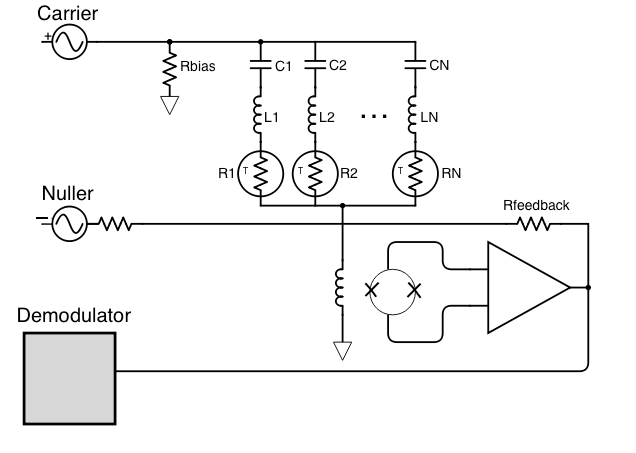
\includegraphics[width=0.6\columnwidth]{figures/dfmux_schematic.png}
\caption{Schematic of readout electronics. 
\label{fig:dfmux} }
\end{center}
\end{figure}
 
%%%%%%%%%%%%%%%%%%%%%%%%%%%%%%%%%%%%%%%%%%%%%%%%%%%%%%%%%%%%%%%%%%%%%%%%%%%%%}}}





%%%%%%%%%%%%%%%%%%%%%%%%%%%%%%%%%%%%%%%%%%%%%%%%%%%%%%%%%%%%%%%%%%%%%%%%%%%%%%%%%
%% Status of Field {{{
%%%%%%%%%%%%%%%%%%%%%%%%%%%%%%%%%%%%%%%%%%%%%%%%%%%%%%%%%%%%%%%%%%%%%%%%%%%%%%%%%
%\section{Status of Field}
%\label{sec:field_status}
%%%%%%%%%%%%%%%%%%%%%%%%%%%%%%%%%%%%%%%%%%%%%%%%%%%%%%%%%%%%%%%%%%%%%%%%%%%%%%%%%
%Some other folks are working on this very same thing, too.
%But. This doesn't even belong here.
% YOU NEED TO KNOW THE STATUS OF THE FIELD, BUT IT IS NOT GOING TO GET A SECTION IN YOUR THESIS.
%%%%%%%%%%%%%%%%%%%%%%%%%%%%%%%%%%%%%%%%%%%%%%%%%%%%%%%%%%%%%%%%%%%%%%%%%%%%%%}}}



%%%%%%%%%%%%%%%%%%%%%%%%%%%%%%%%%%%%%%%%%%%%%%%%%%%%%%%%%%%%%%%%%%%%%%%%%%%%%%%%
% Thesis Overview {{{
%%%%%%%%%%%%%%%%%%%%%%%%%%%%%%%%%%%%%%%%%%%%%%%%%%%%%%%%%%%%%%%%%%%%%%%%%%%%%%%%
%\section{Thesis Overview}
%\label{thesis_overview_section}
%%%%%%%%%%%%%%%%%%%%%%%%%%%%%%%%%%%%%%%%%%%%%%%%%%%%%%%%%%%%%%%%%%%%%%%%%%%%%%%%%
%
%\begin{itemize}
%
%%\item Chapter 1 introduces the analytic goals pursued in this thesis.
%
%\item Chapter 2 briefly presents the history of, and science behind, the
%subjects presented in this thesis.
%
%\item In Chapter 3 the experiment is outlined.
%
%\item Chapter 4 describes the simulation process used in the analysis.
%
%\item Chapter 5 follows the chain of reconstruction software used to obtain
%meaningful results from data.
%
%\item Chapter 6 hashes out the strategy for analysis and presents the data and
%simulated sets that will be used in the analysis.
%
%\item Chapter 7 demonstrates the implementation of the event selection
%processes.
%
%\item In Chapter 8 those events selected in Chapter 7 are analyzed.
%
%\item Chapter 9 presents a final discussion of the analyses presented in the
%thesis.
%
%\end{itemize}
%
%%%%%%%%%%%%%%%%%%%%%%%%%%%%%%%%%%%%%%%%%%%%%%%%%%%%%%%%%%%%%%%%%%%%%%%%%%%%%}}}


